\section{Probabilistic Link Travel Times}
\label{sec:lttestimation} 
The prediction of an event is usually tainted with uncertainty. Therefore, when
predicting link travel times it is not possible to produce an accurate
prediction, since there are too many influencing factors like road conditions,
accidents, weather, time of the day, day of the week or season. The methods we
propose, produce a probabilistic prediction which includes all the effects that
have been observed before (historic data) and are influencing the traffic flow
right now (current data). For example if a street segment has often been the
place of an accident (e.g., every other day between 9.00am and 10.00am) then the
historical data will capture this effect and assign a high probability (e.g.,
50\%) to the prediction that the travel time on that segment will be higher than
usual. In this section we will develop three approaches to estimate
probabilistic link travel times and correlations between them.

Before we continue, we need to introduce and explain a few concepts that will be
used throughout this section. \textit{Start time}, is the time for which we want
to predict the travel time. For example, if we want to know how long it will
take to travel from point $A$ to point $B$ if we leave at 8:00am, then the
\textit{start time} will be 8:00am. \textit{Query time}, is the time at which we
are making the prediction. For example, if the current time is 7:00am and we
want to know how long it will take to travel from point $A$ to point $B$ if we
leave at 8:00am, then the \textit{query time} will be 7:00am. As it was seen in
this example, \textit{start time} and \textit{query time} necessarily are not
the same. We call the difference between the two the \textit{prediction time}.


\textbf{Probabilistic Link Travel Times: } The probabilistic link travel time of a link $(i,j)$ at time $t$, $c_{ij}^t$,
can be represented with two models; discrete or continuous.

% For the discrete representation the link travel time is discretized into into % fixed time units ($\phi$) and each of these time units is associated with a probability. In the continuous case a parametrized function is used that represents the pdf over the link travel time. Common functions which are used in the continuous case are the % normal distribution and the gamma distribution. Figure \ref{fig:models} illustrates the representation of a link travel time in the discrete case by a histogram and in the continuous case by a gamma distribution. To some extent, a discrete problem is more general because probability distributions from real-world applications are often available in discrete forms as probability mass functions . Also, any continuous probability function may be appropriately discretized as a pmf straightforwardly.

To represent the link travel time $c_{ij}^t$ with a continuous \textit{pdf}, an appropriate function is needed. Recent studies suggest that in road networks, the link travel times are normally (e.g. \cite{Seshadri10}) or gamma (e.g. \cite{Zockaei13}) distributed. To the best of our knowledge, no approach exists, to compute the sum of several gamma distributed random variables. Hence, we do not explicitly include the gamma distribution in the present study. In the case of a normal distribution, the random variable $c_{ij}^t$ is characterized by a mean $\mu_{ij}^t$ and a standard deviation $\sigma_{ij}^t$.

%\TODO{[Mohammad] Move to related work}\\Only approximate sampling approaches \cite{Zockaei13} or approaches discretizing the distributions \cite{Nie09b} have been proposed so far for the case where link travel times are assumed to be gamma distributed. In the first case, no extension for the time-dependent and correlated setting exists and the latter case is covered by the discretized approach.

In the discrete case, the link travel time is represented by a discrete probability mass function. Therefore, the time domain has to be discretized. The simplest discretization scheme, known as b-discrete, divides the time domain $T = \{t | t = n\cdot \phi \wedge n \in \NN \}$ evenly into intervals of length $\phi$. The corresponding probability mass function $F_{ij}$ of link travel time $c_{ij}$ reads:

\begin{equation}
	F_{ij}(b) = \begin{cases}\int_b^{b+\phi}f_{ij}(w)dw \qquad b =
	0,\phi,\ldots, (L-1)\phi\\
	\int_b^{\infty}f_{ij}(w)dw \qquad b =
	L \phi\\
	0 \qquad otherwise
	\end{cases} 
\end{equation}
where $L \phi$ is the maximal considered time horizon in the future.

%\TODO{[Mohammad] Maybe move to related work. Can be omitted.}\\
%Let us note that besides the b-discrete discretization scheme other schemes \cite{Nie12} such as the $\alpha$-discrete scheme (where the support is divided such that each interval has the same probability mass $\epsilon$) or the adaptive discretization scheme (where starting from the b-discrete scheme, intervals are consolidated until each interval has a minimum probability mass of $1/L$) where proposed sacrificing some numerical accuracy.

\begin{figure*}
    \centering
    \subfigure[9:00am]{
        \label{fig:900}
        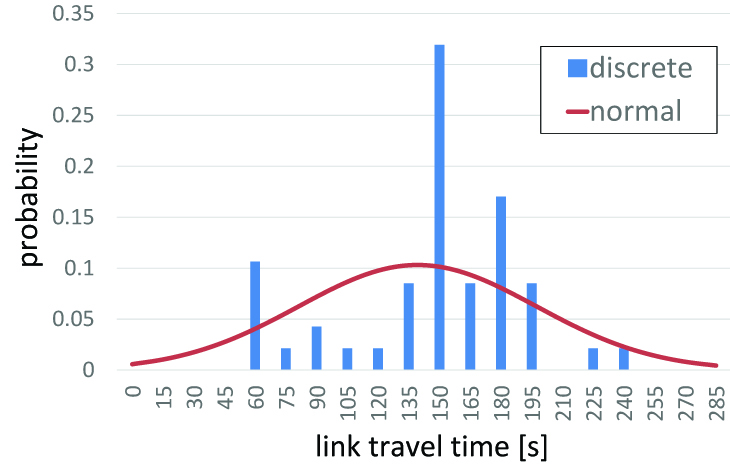
\includegraphics[width = 0.6\columnwidth]{figures/ltt_0900.jpg}
    }
    \subfigure[12:00pm]{
        \label{fig:1200}
        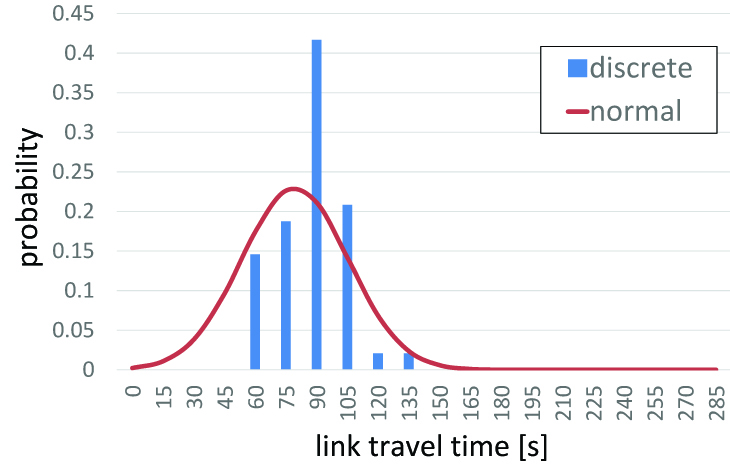
\includegraphics[width = 0.6\columnwidth]{figures/ltt_1200.jpg}
    }
    \subfigure[6:00pm]{
        \label{fig:1800}
        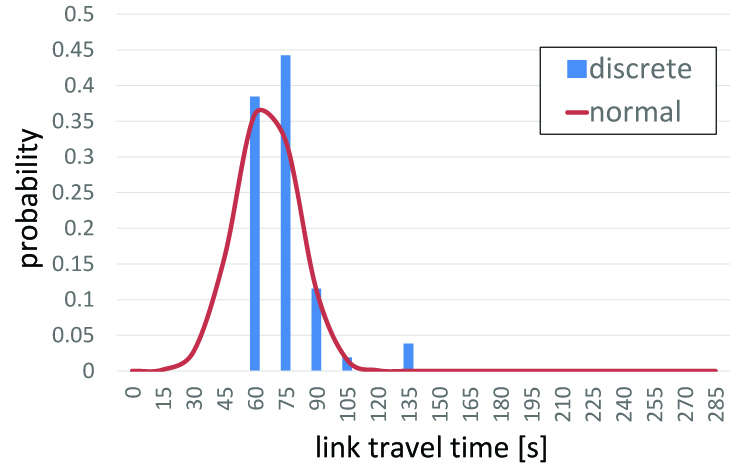
\includegraphics[width = 0.6\columnwidth]{figures/ltt_1800.jpg}
    }
    \caption{Historical model for a street segment for different times of a
    Monday}\label{fig:ltt}
\end{figure*}


%\TODO{[Mohammad] Correlations are not required in this section. Either move it to an appropriate section or remove completely.}\\
%\textbf{Correlations between Link Travel Times: } The assumption that travel times of two links are independent from each other is questionable in a real-world traffic network. For example, given a heavily congested link (resulting in a high travel time), the adjacent link is usually also congested to a similar degree. This simple observation illustrates that integrating some kind of correlation in the model may yield a more exact representation of reality. Again we differentiate between the
%discrete and the normally distributed case:

% For the continuous case under the assumption of normally distributed link travel
% times, we compute a correlation coefficient $\rho_{ij-kl}$ for the correlation
% $corr(c_{ij},c_{kl})$ of any pair $((i,j), (k,l))$ of edges in the graph.
% 
% With the discrete case, we model correlation in the following manner. We assume
% that link travel times may follow two different distributions depending on the
% condition of the link. A link may either be non-congested (State-0) or congested
% (State-1) where each of these two states is then associated with its own
% \textit{pmf}. The correlation between the states of adjacent links are taken
% into account by introducing conditional probabilities $\alpha^{uv}_{ij}$,
% meaning the probability of having link $(i,j)$ in state $v$, if the link leading
% to node $i$ is  in state $u$. This form of correlation allows only for
% expressing correlation between adjacent links, but is adopted by a variety of
% works, hence we follow this model.

% \begin{figure}
%     \centering
%     \subfigure[discrete pdf]{
%         \label{fig:discrete}
%         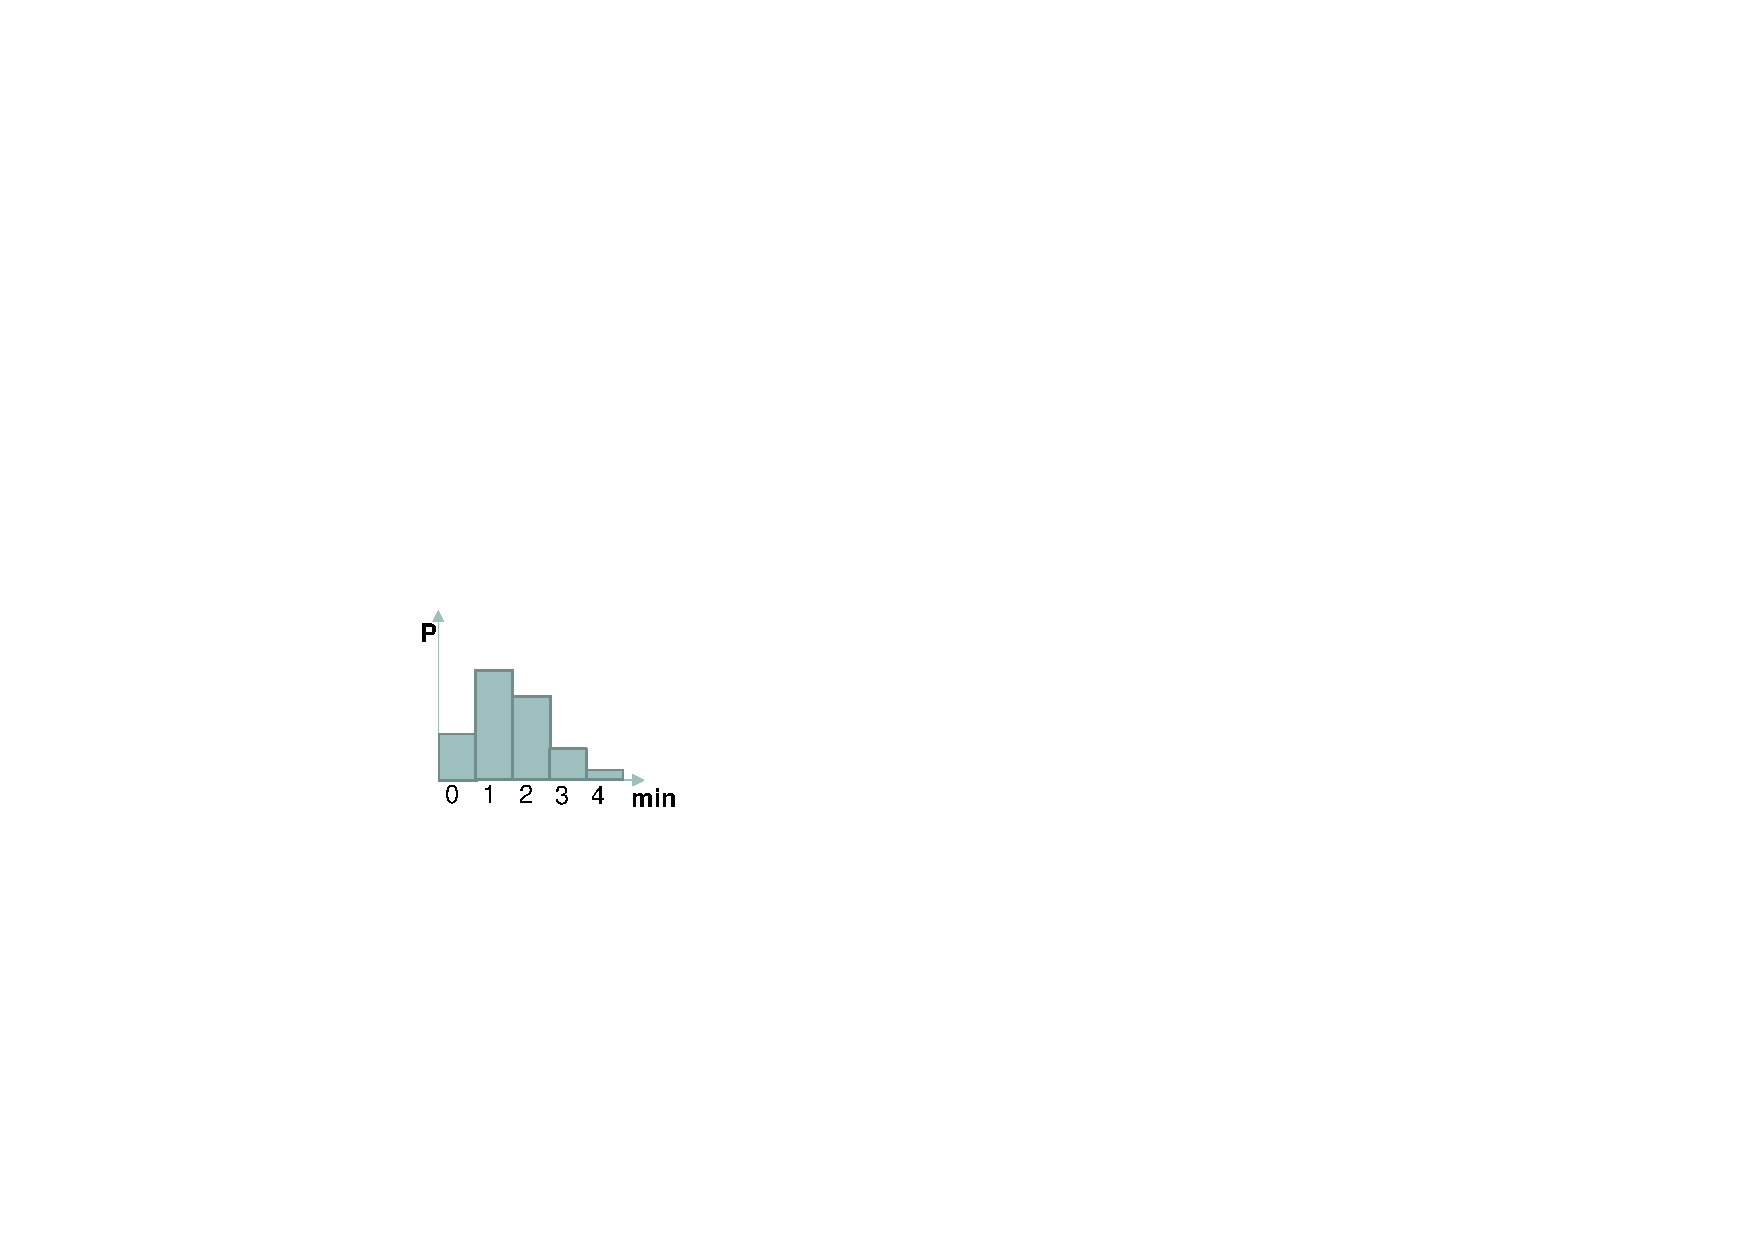
\includegraphics[width = 0.3\columnwidth]{figures/pdf_discrete.pdf}
%     }
%     \subfigure[continuous pdf]{
%         \label{fig:continuous}
%         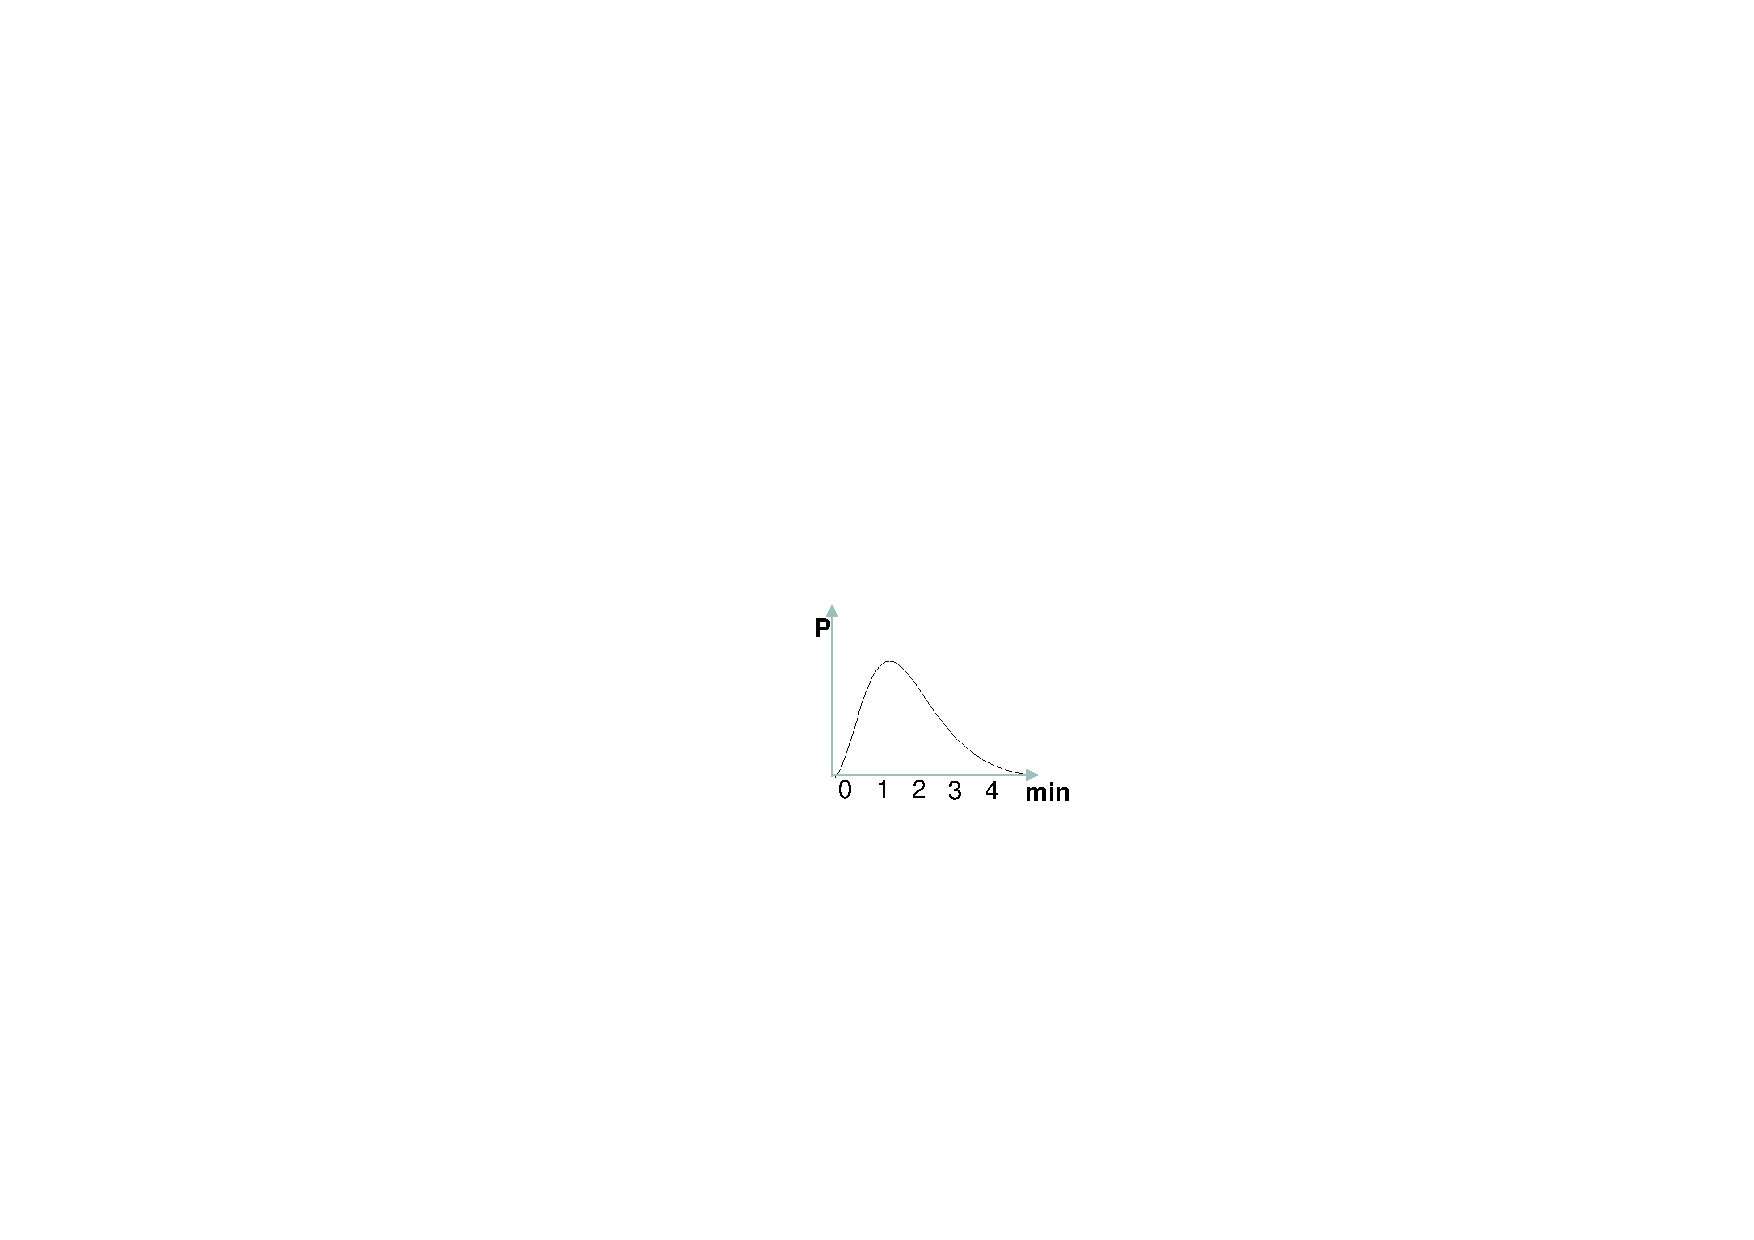
\includegraphics[width = 0.3\columnwidth]{figures/pdf_gamma.pdf}
%     }
%     \subfigure[ltt at rush hour]{
%         \label{fig:traffic}
%         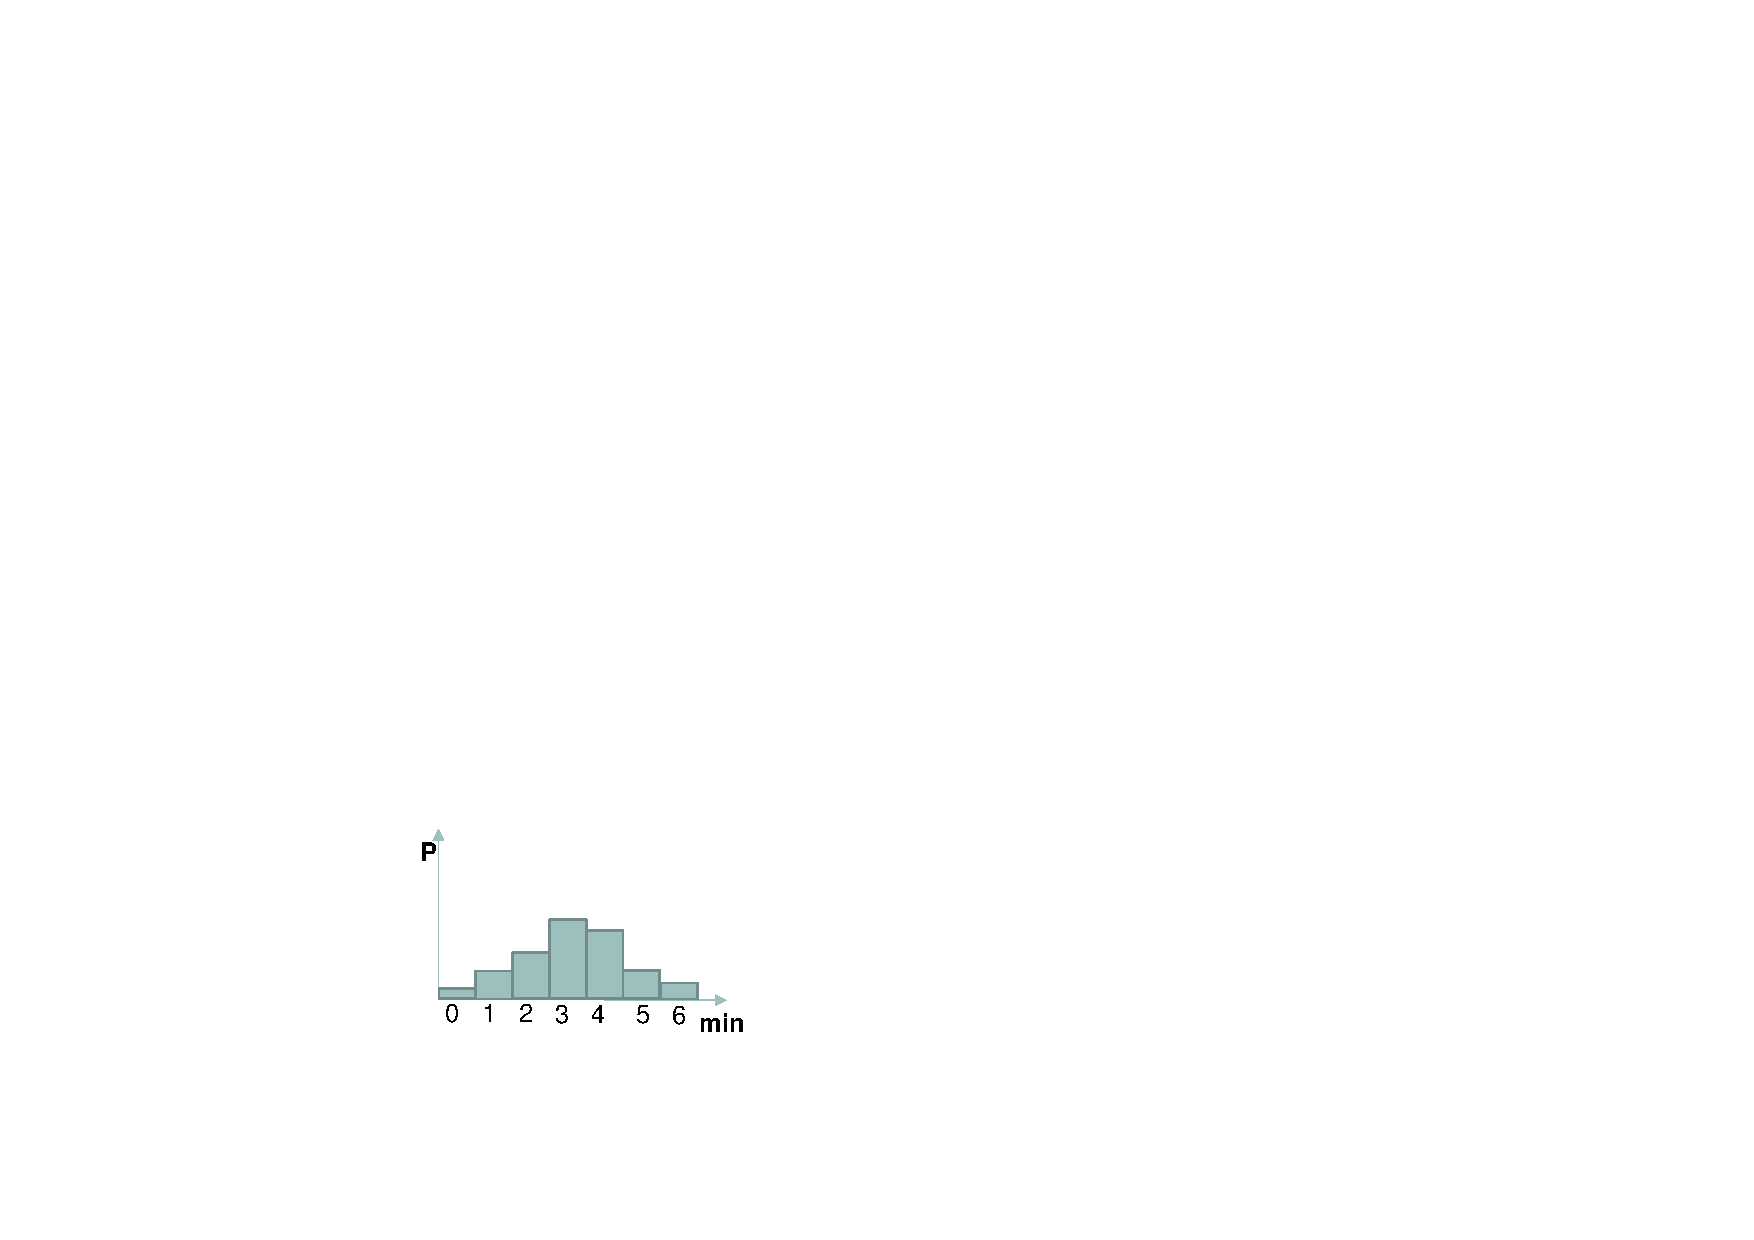
\includegraphics[width = 0.3\columnwidth]{figures/pdf_traffic.pdf}
%     }
%     \caption{Representation of link travel times}
%     \label{fig:models}
% \end{figure}

% The last section summarized existing works on reliable shortest-path search under the consideration of uncertainty of link travel times with a particular focus on the computation of the pdf representing the path travel time of a given path. However none of the mentioned works describes how to generally obtain the uncertain link travel times. Thus to the best of our knowledge there does neither exist an evaluation of the effectiveness of such approaches nor a comparison of several approaches with respect to the expected accuracy. We wish to close this research gap and provide methods how to obtain adequate uncertain link travel times and additional necessary parameters in order to provide meaningful outcomes. In the following we thus aim at obtaining a pdf (or pmf) representing $c_{ij}^t$ and parameters for describing the correlation $corr(c_{ij},c_{kl})$ between two edges $(i,j)$ and $(k,l)$.

% In order to allow for accurate parameter estimation we assume that the following data is present:
% \begin{itemize}
%   \item The graph of the road network to consider $G(V,E)$.
%   \item For each edge $(i,j) \in G$ in the network historical data about the
%   link travel time $c_{i,j}^t, t \in H = \{-A\phi, (-A+1)\phi, \ldots,
%   -\phi\}$.
%   \item For each edge $(i,j) \in G$ in the network the current link travel time
%   $c_{ij}^0$.
% \end{itemize}

In the remainder of this section, we will discuss our techniques to generate probabilistic link travel-times.

\subsection{Prediction through Historical Data}
\label{subsec:historical}
To obtain a \textit{pdf} representing $c_{ij}^t$ for a time $(t>t_c)$, where $t_c$ is the current time, a
simple approach is to use the available historical data. We define the set of historical data as $H = \{h | h < t_c\}$.
Let us note that the link travel time $c_{ij}^h$ where $ h < t_c$ is not a random variable but a certain value which is known. In order to predict the travel time for time $t > t_c$ more accurately, we only consider a subset of historical data, $H^t \subset H$, with similar characteristics to time $t$. For example, if we want to predict the behaviour of edge $(i,j)$ at 9:00am for the next Tuesday, an adequate set $H^t$ might consist of data points $h$, where $h$ is 9:00am on a Tuesday in the last year. The travel time $c_{i,j}^h$ corresponding to last Friday 10:00pm might on the other hand, not be valuable in the prediction.

How to choose a set $H^t$ highly depends on the characteristics of the underlying traffic network. We use the results in \cite{Pan12} for choosing the appropriate $H^t$ for each start time. For a specific \textit{time of day} during a weekday, $H^t$ consists of data points corresponding to the same \textit{time of day} during \textbf{\textit{any}} weekday. For example, if the start time is 9:00am on this Tuesday, $H^t$ will consist of data points at 9:00am during Mondays, Tuesdays, Wednesdays, Thursdays and Fridays. The assumption is that traffic patters during weekdays are similar. More details can be found in \cite{Pan12}.

For continuous representation of the link travel time, we assume normal distribution with the following parameters
\begin{gather}
	\mu_{ij}^t = \frac{1}{|H^t|}\sum_{h\in H^t} c_{i,j}^h\\ 
	(\sigma_{ij}^t)^2 = \frac{1}{|H^t|}\sum_{h\in H'} (c_{ij}^h-\mu_{ij}^t)^2\\
	\rho_{ij-kl} = \frac{\sum_{h\in H^t} (c_{ij}^h - \mu_{ij}) (c_{kl}^h -
	\mu_{kl})}{(|H^t-1| \sigma_{ij} \sigma_{kl})}
\end{gather}

where $\rho$ is the Pearson correlation coefficient \cite{Soper17}

For the case of discrete representation through a \textit{pmf} we set
\begin{gather}
F_{ij}^t(b) = \frac{1}{|H^t|}\sum_{h\in H^t} I(c_{ij}^h = b)
\end{gather}
where $I(c_{ij}^h = b)$ is an indicator variable which is 1 if $c_{ij}^h =
b$ and 0 otherwise. The \textit{pmf} of each edge is thus given by a histogram
assigning for each possible travel time of the edge a probability corresponding to its
proportional occurrence in the historical data. 

%For discrete correlated link travel times as processed in the methods described in \cref{sec:methods}, it is necessary to provide two link travel time distributions $F_{ij}^t(b, 0)$ (for the uncongested state) and $F_{ij}^t(b, 1)$ (for the congested state). Additionally, the conditional probabilities $\alpha^{uv}_{ij}$ have to be at hand. Since none of the recent studies \cite{Waller02,Fan05} describe how to obtain these parameters, we propose a feasible approach. The basic idea is to define the two states of a link by the travel time itself. Thus we introduce a parameter $\kappa_{ij}$. A travel time $c_{ij}^t$ above or below that threshold implies that the link is in the normal state or the congested state.
%\begin{gather}
%	F_{ij}^t(b, 0) = \begin{cases}F_{ij}^t(b) \qquad \text{if } b %\geq
%	\kappa_{ij}\\
%	0 \qquad otherwise
%	\end{cases} \\
%	F_{ij}^t(b, 1) = \begin{cases}F_{ij}^t(b) \qquad \text{if } b 
%< \kappa_{ij}\\
%	0 \qquad otherwise
%	\end{cases}
%\end{gather}

%The correlation parameter between a link $(i,j)$ and its incoming link $(k,i)$ can then be computed based on the historical data as follows:

%\begin{equation}
%	\alpha^{00}_{ij} = \frac{\sum_{h\in H^t} I(c_{ij}^h \geq
%	\kappa_{ij} \wedge c_{ki}^h \geq
%	\kappa_{ki})}{|H^t|}
%\end{equation}

%The values of $\alpha^{01}, \alpha^{10}$ and $\alpha^{11}$ can be computed analogously by adapting the conditions in the indicator function. Note that $\alpha^{uv}_{ij}$ can have different values for different incoming links $(k,i)$. However, in the scope of this work the link $(i,j)$ is located on a given path of interest and has thus a unique incoming link.


\cref{fig:ltt} shows the discrete and continuous models of a typical inbound street segment of the network with a length of 1 mile for different times of the day. Based on the observation of historic patterns, in the morning a lot of traffic passes through this link. More traffic, intuitively, implies a higher probability of accidents which explains the rather large variation in the link travel time. At noon the traffic is
reduced and in the evening the link travel time has the least amount of traffic, yielding the fastest travel time and in this case also the smallest variance. The figure also shows that the use of a normal distribution might not always adequately represent the link travel time.

We end this subsection with a note on \textit{query time} and \textit{prediction time}. When only historic data is used for prediction, the concept of prediction time becomes irrelevant. This means that if we are predicting for start time set to 9:00am today and we only use historic data, whether the query time is 7:00am or 8:00am does not make any difference since we only use $H^t$ corresponding to the start time to build the model. Prediction time and query time become important once we take the \textit{current situation} into account when building the prediction model which we will discuss in the following. 

\subsection{Historical Data and Current Situation}
The technique discussed in \cref{subsec:historical} provides link travel time
distributions only based on historical data. These estimations may be a good choice if the time $t$, for which the link travel time has to be predicted, is reasonably far (e.g., more than several hours) in the future. However, it may not be sufficient to capture current (and near future) traffic conditions with high confidence. For example, if we want to predict the travel time for 5 minutes later, the current situation of the road network might be more relevant than the historic data. Therefore, we present two parameter estimation methods, incorporating both, the historical as well as the current link travel times of edges.

\subsubsection{Prediction through Linear Interpolation}
\label{subsec:LI}
The intuition of this approach is that 
\begin{itemize}
  \item for a start time $t$ which is far in the future, the historical prediction (cf \cref{subsec:historical}) is expected to yield a good prediction performance and
\item for the start time $t = t_c$, the current situation yields the best "prediction".
\end{itemize}

Thus, for a start time $t$ which is in the relatively near future, we argue that both, the historical as well as the current situation should influence the prediction. The closer the time $t$ is to $t_c$ (smaller prediction time) the more weight the current situation should have and vice versa. As the prediction time increases, we eventually get to a point where the current situation should loose it's influence. Towards this end we define a threshold parameter $\tau$, which defines the time-horizon in which the current situation has an influence on the prediction. Using a small time horizon $\tau$ is basically valuing the historic data, whereas setting $\tau$ to a larger value
puts more weight on the current situation. We also define $\theta \in [0,1]$ as the relative importance of the current situation in the estimation. $\theta$ depends on the prediction time and is computed as:
\begin{equation}
\theta = \frac{t-t_c}{\tau}
\end{equation}
where, as explained earlier, $t-t_c$ is the prediction time.

For continuous representation of link travel times, we estimate the parameters of the normal distribution as:

\begin{gather}
	\mu_{ij}^t = \frac{t - t_c}{\tau}\cdot\frac{1}{|H^t|}\sum_{h\in H^t} c_{i,j}^h
	+ (1-\frac{t - t_c}{\tau})\cdot c_{i,j}^{t_c}\\
	(\sigma_{ij}^t)^2 = (\frac{t - t_c}{\tau})^2 \cdot \frac{1}{|H^t|}\sum_{h\in H^t}
	(c_{ij}^h-\mu_{ij}^t)^2
\end{gather}

In particular, we perform a linear interpolation between the current link travel time, and the summarized historical link travel time in order to find the link travel time to be estimated. \cref{fig:interpolation} illustrates this concept, where  $\theta = 0.5$ and thus the expected value of the prediction is the average of the current situation and the predicted value by the historical approach. Accordingly, the standard deviation of the historical prediction is cut by half.

\begin{figure}[h]
    \centering
    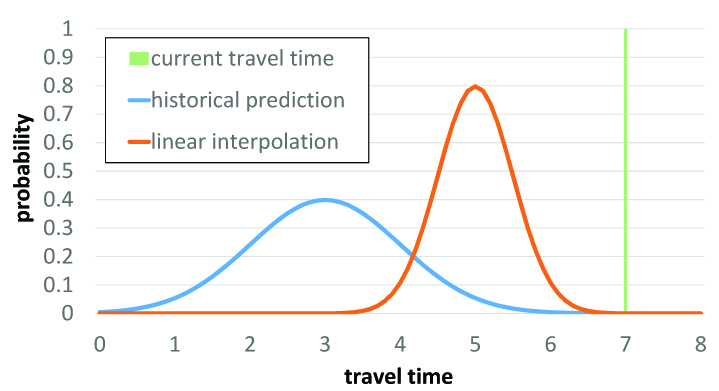
\includegraphics[width=0.80\columnwidth]{figures/tt_interpolation.jpg}
    \caption{Linear interpolation of ltt}
    \label{fig:interpolation}
\end{figure}

In the case of discrete link travel times, we adapt the same concept and obtain the following parameters.

\begin{gather}
F_{ij}^t(b) = \frac{1}{|H^t|}\sum_{h\in H^t} I(\lceil\frac{t - t_c}{\tau} \cdot 
c_{ij}^h + (1-\frac{t - t_c}{\tau})\cdot c_{i,j}^{t_c}\rceil^\phi = b)
\end{gather}

where $\lceil x \rceil^\phi$ rounds $x$ up to the next multiple of $\phi$ and $I()$ is the indicator function.

\subsubsection{Prediction through Similar Historical Data}
\label{subsec:SH}
The third and final approach we propose is based on the idea that the current situation is a crucial indicator of how the travel time of a link will develop in the future. In this approach we use the current situation to further restricts the set $H^t$. Specifically we only include times $h \in H^t$, for which link $(i, j)$ had a travel time similar to the current situation at time $h-(t-t_c)$. In this context, we define similarity by a percentage threshold $\lambda$, which represents the deviation from the current travel time.
To illustrate this idea, we provide an example. Assume we are predicting the travel time for link $l$ where the query time is 7:00am and the start time is 8:00am. We only consider the data points at 8:00am from days where the traffic at 7:00am was similar to today. For example, if the current travel time over link $l$, is 5 minutes and $\lambda = 0.2$, we only consider days where the travel time over link $l$ is somewhere between 4 minutes and 6 minutes.

We can formally define the further restricted set $H_{i,j}^t$ as:

\begin{equation}
H_{i,j}^t = \{h|h \in H^t \wedge \left| \frac{c_{i,j}^{t_c} - c_{i,j}^{h-t_p}}{c_{i,j}^{t_c}} \right| \leq \lambda \}  
\end{equation}

where $t_p$ is the prediction time.

The value of $\lambda$ affects the prediction result. Setting $\lambda$ too small might result in not enough sample points. This can cause problems like over fitting the model. On the other hand setting $\lambda$ too large yields the historical prediction approach. In \cref{sec:experiments} we test with different values of $\lambda$ to find the optimal value for this parameter. 


